\documentclass[a4j]{jsreport}
\usepackage[dvipdfmx]{graphicx}
\usepackage{multicol}
\usepackage{amsmath}
\usepackage{siunitx}
<<<<<<< HEAD
\usepackage[version=4]{mhchem}
\usepackage{url}


\graphicspath{{./figure/}}
\bibliographystyle{jplain}


\newcommand{\diff}{\mathrm{d}}
\DeclareSIUnit{\solventgram}{\si{\gram}\text{-solvent}}


\begin{document}

=======

\bibliographystyle{jplain}

\title{トルエンの空気酸化による安息香酸の製造}
\author{荊尾太雅 \and 宮本奏汰}

\newcommand{\diff}{\mathrm{d}}

\begin{document}
>>>>>>> miyamoto
% 表紙
\begin{titlepage}
\vspace{5cm}
\centering
{\Huge トルエンの空気酸化による安息香酸の製造}\\
\vspace{2cm}
\centering
{\Large 1講座 移動現象論分野}\\
\vspace{0.5cm}
\centering
<<<<<<< HEAD
{\large 荊尾太雅 , 宮本奏汰}\\
=======
{\large 荊尾太雅  宮本奏汰}\\
>>>>>>> miyamoto
\vspace{3cm}
\begin{table}[htbp]
    \begin{center}
        \begin{tabular}[htbp]{ll}
<<<<<<< HEAD
            \multicolumn{2}{c}{{\LARGE keyword}}\\
            {\Large 空気酸化}&{\Large Air oxidation}\\
            {\Large 気液反応}&{\Large Gas-liquid reaction}\\
            {\Large 晶析}&{\Large Crystallization}\\
            {\Large 多変数同時全体最適化}&{\Large Multi-variable simultaneous optimization}\\
=======
            \multicolumn{2}{l}{{\LARGE keyword}}\\
            {\Large 空気酸化}&{\Large Air oxidation}\\
            {\Large 気液反応}&{\Large Gas-liquidreaction}\\
            {\Large 晶析}&{\Large Crystallization}\\
            {\Large 多変数全体同時最適化}&{\Large Multi-variable simultaneous optimization}\\
>>>>>>> miyamoto
            {\Large }&{\Large air}\\
        \end{tabular}
    \end{center}
\end{table}
\end{titlepage}

<<<<<<< HEAD

=======
>>>>>>> miyamoto
\pagenumbering{roman}
\setcounter{tocdepth}{2}
\tableofcontents


% 本文
\pagenumbering{arabic}
\chapter{緒言}
安息香酸は,主としてフェノールの原料となる他,その塩が食品や化粧品などの添加物として広く利用されている.
<<<<<<< HEAD
2014年には世界全体で48万トンが製造されており,新興国での需要から,2024年には生産量が64万トンとなると見込まれている.
=======
2014年には世界全体で 万トンが製造されており,新興国での需要から,2024年には生産量が 万トンとなると見込まれている.
>>>>>>> miyamoto
そこで,私たちは原料として安価なトルエンを使用し,空気酸化することで安息香酸を製造するプロセスを
題材とし,本プロセス設計演習において検討することにした.

\newpage
\chapter{プロセスの概要}
\section{プロセスの概要}
本設計で対象とするのは,トルエンを空気酸化することにより安息香酸を製造するプロセスである.
<<<<<<< HEAD
プロセス全体の概略図を図\ref{プロセス全体のの概略図}に示す.
\begin{figure}[htbp]
    \label{プロセス全体のの概略図}
    \begin{center}
        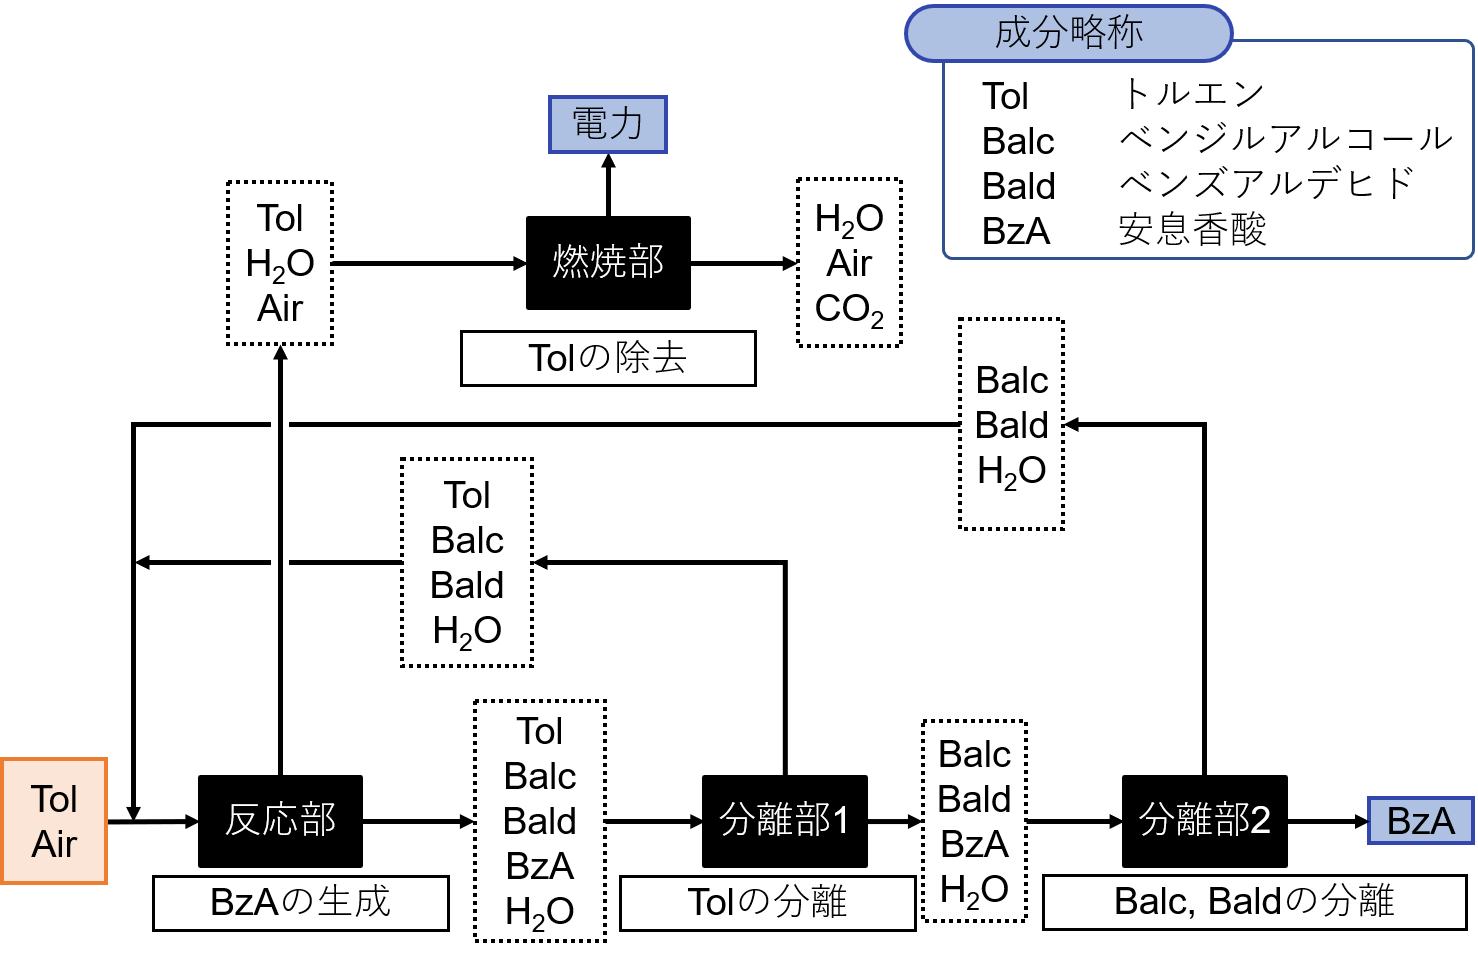
\includegraphics[scale=0.5]{processOutline.png}
        \caption{プロセス全体の概略図}
    \end{center}
\end{figure}

\section{設計条件}
プロセスを設計するにあたり,以下の6つの条件を設定した.
\begin{enumerate}
    \item 生産要求は,99.0wt\%以上の安息香酸を年2万トンとする.\\
    \item 工場の稼働時間は,1日24時間,年300日とする.\\
    \item 原料として,純度100\%のトルエンおよび,組成を窒素79mol\%酸素21mol\%とする空気を用いる.
             ただし,両原料は25℃,1barで供給されるものとする.\\
    \item 減価償却期間は7年である.\\
    \item 圧力損失,熱損失,制御系については考慮しない.\\
    \item HYSISを用いての物性推算はUNIQUAC式によって行った.
=======
プロセス全体の概略図を以下に示す.

\section{設計条件}
\begin{enumerate}
    \item 生産要求は,99.0wt\%以上の安息香酸を年2万トンとする.\\
    \item 工場の稼働時間は,1日24時間,年300日とする.\\
    \item 原料として,純度100\%のトルエンおよび,組成を窒素79mol\%酸素21mol\%とする空気を用いる.\\
    \item ただし,原料は25℃,1barで供給されるものとする.\\
    \item 減価償却期間は7年である.
>>>>>>> miyamoto
\end{enumerate}

\newpage
\chapter{反応部}
<<<<<<< HEAD

反応部の概略図を図 \ref{反応部設計結果の概略図} に示す.
\begin{figure}[htbp]
    \label{反応部設計結果の概略図}
    \begin{center}
        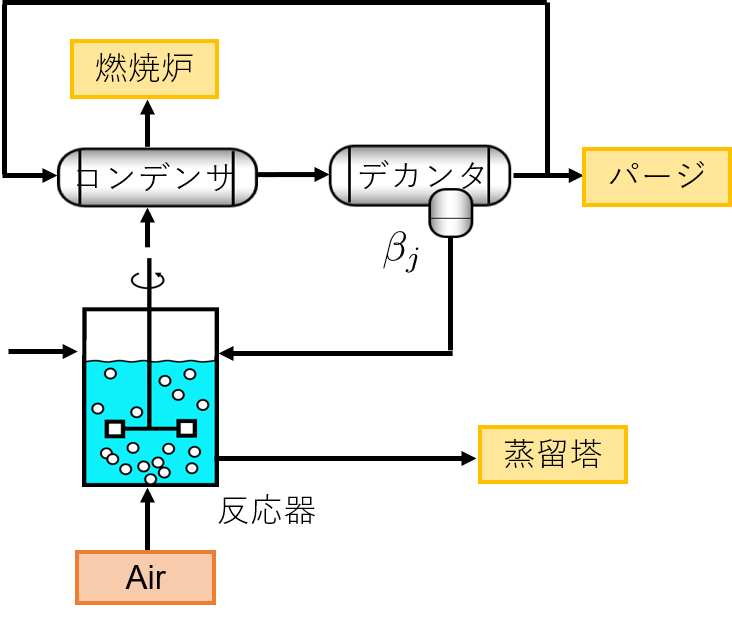
\includegraphics[scale=0.7]{ReactionSection.png}
        \caption{反応部概略図}
    \end{center}
\end{figure}

\section{反応機構}
今回用いた反応は以下の4つである.
\begin{center}
\begin{tabular}{lcrlll}
  \ce{Tol}  & + & \ce{O2}     & \ce{-> Bald + H2O} & $r_1 = k_1 \cdot C_\text{Tol}$  & $\varDelta _\mathrm{r} H_1 = -385.23$ \, \si{\kilo \joule \per \mole} \\
  \ce{Tol}  & + & 1/2 \ce{O2} & \ce{-> Balc}       & $r_2 = k_2 \cdot C_\text{Tol}$  & $\varDelta _\mathrm{r} H_2 = -167.30$ \, \si{\kilo \joule \per \mole} \\
  \ce{Balc} & + & 1/2 \ce{O2} & \ce{-> Bald + H2O} & $r_4 = k_3 \cdot C_\text{Balc}$ & $\varDelta _\mathrm{r} H_3 = -317.30$ \, \si{\kilo \joule \per \mole} \\
  \ce{Bald} & + & 1/2 \ce{O2} & \ce{-> BzA}        & $r_3 = k_4 \cdot C_\text{Bald}$ & $\varDelta _\mathrm{r} H_4 = -298.20$ \, \si{\kilo \joule \per \mole}
\end{tabular}
\end{center}

ただし,トルエンをTol,ベンジルアルコールをBalc,ベンズアルデヒドをBald,安息香酸をBzAとしている.これらの反応は全て参加反応であり,触媒には,酸化剤であるモリブデン酸マンガン\ce{MnMoO4}を用いることとした.これらの反応の反応速度定数は,表\ref{}のようである\cite{}.
\begin{table}
  \centering
  \label{}
  \caption{}
  \begin{tabular}{ccccc}
    \hline
    & $k_1$ & $k_2$ & $k_3$ & $k_4$ \\
    \hline
    $\ln A_j \, [\si{-}]$ & 17.93 & 20.63 & 15.40 & 19.70 \\
    $E_j \, [\si{\kilo \joule \per \mole}]$ & 69.53 & 81.39 & 56.99 & 71.44 \\
    \hline
  \end{tabular}
\end{table}
=======
反応部の概略図を以下に示す.

\section{反応機構}
>>>>>>> miyamoto

\section{反応器選定}
流通式の気液反応器の種類には,拡散速度に対して不利な順に,気泡塔,気液攪拌槽,充填塔などがある.
最大反応速度と最大拡散速度の比を表す八田数を事前に概算し,
参考文献\cite{化工便覧}の選定基準に基づき,八田数が0.1より小さいなら気泡塔,
5より大きければ充填塔,中間域ならば気液攪拌槽を選択した.
今回は気液攪拌槽型反応器を選択した.実際のプロセスでは気泡塔も選択される.\\
<<<<<<< HEAD
八田数の定義式
=======
>>>>>>> miyamoto
\begin{equation}
    \gamma = \frac{\text{(最大反応速度)}}{\text{(最大拡散速度)}} = \frac{(C_\mathrm{B}kD_\mathrm{B})^{1/2}} {k_\mathrm{L}}
\end{equation}

\section{設計方程式}
液相は完全混合状態として,気相は鉛直方向に向かう押し出し流れとなっているとして設計を行った.
<<<<<<< HEAD
用いた仮定は以下のようである.
\begin{itemize}
    \item[-] 気相は水平方向に一様な濃度分布を持つ.
    \item[-] 気相側境膜抵抗は無視できる
    \item[-] 液相は完全混合状態である.
    \item[-] 窒素,酸素はヘンリー則に従い,その他の物質はラウール則に従う.
\end{itemize}
以上の仮定および,蒸発油分を還流する機構を含めて,設計方程式(\ref{液相物質収支式}),(\ref{気相物質収支式})を立式した.\\
\begin{equation}
    \label{液相物質収支式}
    0 = F^\text{in}_{\text{liq},j} - F^\text{out}_{\text{liq},j} - (1-\beta_j) k_\mathrm{L}a
    \int^{V_\text{tot}}_0(C_j - C^\text{sat}_j) \diff V + r_j V_\mathrm{L}
\end{equation}
\begin{equation}
    \label{気相物質収支式}
    \frac{ \diff F_{\text{gas},j}}{\diff V} = k_\mathrm{L}a (C_j - C^\text{sat}_j)
\end{equation}

\section{物質移動容量係数の推算}
=======
用いた仮定は以下のようになる.
\begin{itemize}
    \item[-] 気相は水平方向に一様な濃度分布を持つ.
    \item[-] 気相側境膜抵抗は無視できる・
    \item[-] 液相は完全混合状態である.
    \item[-] 窒素,酸素はヘンリー則に従い,その他の物質はラウール則に従う.
\end{itemize}
以上の仮定および,蒸発油分を還流する機構を含めて,設計方程式を立式した.\\
\begin{equation*}
    0 = F^\text{in}_{\text{liq},j} - F^\text{out}_{\text{liq},j} - (1-\beta_j) k_\mathrm{L}a
    \int^{V_\text{tot}}_0(C_j - C^\text{sat}_j) \diff V + r_j V_\mathrm{L}
\end{equation*}
\begin{equation*}
    \frac{ \diff F_{\text{gas},j}}{\diff V} = k_\mathrm{L}a (C_j - C^\text{sat}_j)
\end{equation*}

\section{物質移動容量係数の推算}
% TODO: 書式の統一
>>>>>>> miyamoto
物質移動容量係数の推算に用いた各相関式を記す.

液相側物質移動係数の相関式\\
小気泡の場合
\begin{equation}
<<<<<<< HEAD
    k_\mathrm{L} = 0.31Sc_\mathrm{L}^{-2/3}(g \varDelta \rho \mu_\mathrm{L}/\rho_\mathrm{L}^2)^{1/3}
\end{equation}
大気泡の場合
\begin{equation}
    k_\mathrm{L} = 0.42Sc_\mathrm{L}^{-1/2}(g \varDelta \rho \mu_\mathrm{L}/\rho_\mathrm{L}^2)^{1/3}
=======
    k_\mathrm{L} = 0.31Sc_\mathrm{L}^{-2/3}(g \Delta \rho \mu_\mathrm{L}/\rho_\mathrm{L}^2)^{1/3}
\end{equation}
大気泡の場合
\begin{equation}
    k_\mathrm{L} = 0.42Sc_\mathrm{L}^{-1/2}(g \Delta \rho \mu_\mathrm{L}/\rho_\mathrm{L}^2)^{1/3}
>>>>>>> miyamoto
\end{equation}
比表面積の相関式
\begin{equation}
    a = 1.44 \left( \frac{P_\mathrm{V}^{0.4} \rho_\mathrm{L}^{0.2} }{ \sigma^{0.6}} \right) \left( \frac{u_\mathrm{G}}{u_\mathrm{t}} \right)^{0.5} \left( \frac{P_\mathrm{T}}{P_\mathrm{G}} \right) \left( \frac{\rho_\mathrm{G}}{\rho_\mathrm{a}} \right)^{0.16}
\end{equation}

上記の2式を利用するために用いた相関式を以下に記す.

ガスホールドアップの相関式
\begin{equation}
    \varepsilon_{{\mathrm G}} = \left( \frac{u_{{\mathrm G}}\varepsilon_{{\mathrm G}}}{u_{{\mathrm t}}} \right) + 0.000216 \times \left( \frac{P_\mathrm{V}^{0.4} \rho_\mathrm{L}^{0.2} }{ \sigma^{0.6}} \right) \left( \frac{u_\mathrm{G}}{u_\mathrm{t}} \right)^{0.5} \left( \frac{P_\mathrm{T}}{P_\mathrm{G}} \right) \left( \frac{\rho_\mathrm{G}}{\rho_\mathrm{a}} \right)^{0.16}
\end{equation}
気泡の体積平均径の相関式
\begin{equation}
    d_\mathrm{vs} = 4.15 \left( \frac{\sigma^{0.6}}{P_\mathrm{V}^{0.4} \rho_\mathrm{L}^{0.2}} \right) \left( \frac{P_\mathrm{G}}{P_\mathrm{T}} \right) \left( \frac{\rho_\mathrm{a}}{\rho_\mathrm{G}} \right) ^{0.16} \varepsilon_\mathrm{G}^{0.5} + 0.0009
{}\end{equation}
気泡の終末速度の相関式
\begin{equation}
    u_\mathrm{t} = \left( \frac{4\varDelta \rho g d_\mathrm{vs}}{3C_\mathrm{D} \rho_\mathrm{L}} \right)^{0.5}
\end{equation}

さらに,上記の相関式を利用するために用いた物性値の推算式,および変数の定義式などの諸式を以下に記す.

抗力係数の相関式
\begin{equation}
    C_\mathrm{D} = \max \left[ \frac{24}{Re}(1+0.15Re^{0.687}), \, \frac{8}{3} \frac{Eo}{Eo+4} \right]
\end{equation}
拡散係数の推算\\
wilke-changの式
\begin{equation}
    D_{12} = \frac{2.946\times 10^{-11}(\beta M_{\mathrm{r,2}})^{1/2} T} {\mu_2 V_{\mathrm{b},1}^{0.6}}
\end{equation}
Einstin-Stokesの式
\begin{equation}
    \frac{D \mu}{T} = \text{const}
\end{equation}

界面張力の推算\\
界面張力の温度依存性に関する相関式
\begin{equation}
    \sigma \propto \{ 1-(T/T_\mathrm{c}) \}^n
\end{equation}

気泡レイノルズ数の定義式
\begin{equation}
    Re = \frac{\rho_\mathrm{L}u_\mathrm{t} d_\mathrm{vs}}{\mu_\mathrm{L}}
\end{equation}
エトベス数の定義式
\begin{equation}
<<<<<<< HEAD
    Eo = \frac{g \varDelta \rho d_\mathrm{vs}^2}{\sigma}
\end{equation}

以上の式を用いる際にデータとして,参考文献[]からトルエンの界面張力$\sigma=0.81 \,\si{\newton \per \square \metre}$とした.

\section{反応器設計結果}
最終結果における反応器の詳細を表\ref{反応器設計結果の表}に示す.
\begin{table}[htbp]
    \label{反応器設計結果の表}
    \caption{反応器設計結果}
    \begin{center}
        \begin{tabular}{lc}
            \hline
            \multicolumn{1}{c}{項目} & 値 \\
            \hline
            反応器内圧力 \, [\si{bar}] & 7.00 \\
            反応器内温度 \, [\si{\degreeCelsius}] & 170 \\
            反応器体積 \, [\si{\cubic \metre}] & 14.6 \\
            気液総体積 \, [\si{\cubic \metre}] & 8.25 \\
            ガスホールドアップ \, [\si{-}] & 0.115  \\
            液平均滞留時間 \, [\si{\hour}] & 0.478  \\
            物質移動容量係数 \, [\si{\per \second}] & 0.470  \\
            液相物質移動係数 \, [\si{\metre \per \second}] & 0.00172 \\
            比界面積 \, [\si{\per \metre}] & 273 \\
            反応器空間率 \, [\si{-}] & 0.435 \\
            総攪拌動力 \, [\si{\kilo \watt}] & 8.25 \\
            気泡体積平均径 \, [\si{\milli \metre}] & 2.53 \\
            エトベス数 \, [\si{-}] & 1480 \\
            気泡レイノルズ数 \, [\si{-}] & 1170 \\
            \hline
        \end{tabular}
    \end{center}
\end{table}

\section{反応部設計結果}
最適化後の最終結果における反応部の物質収支を図\ref{反応部設計結果の図}中に示す.
\begin{figure}[htbp]
    \label{反応部設計結果の図}
    \begin{center}
        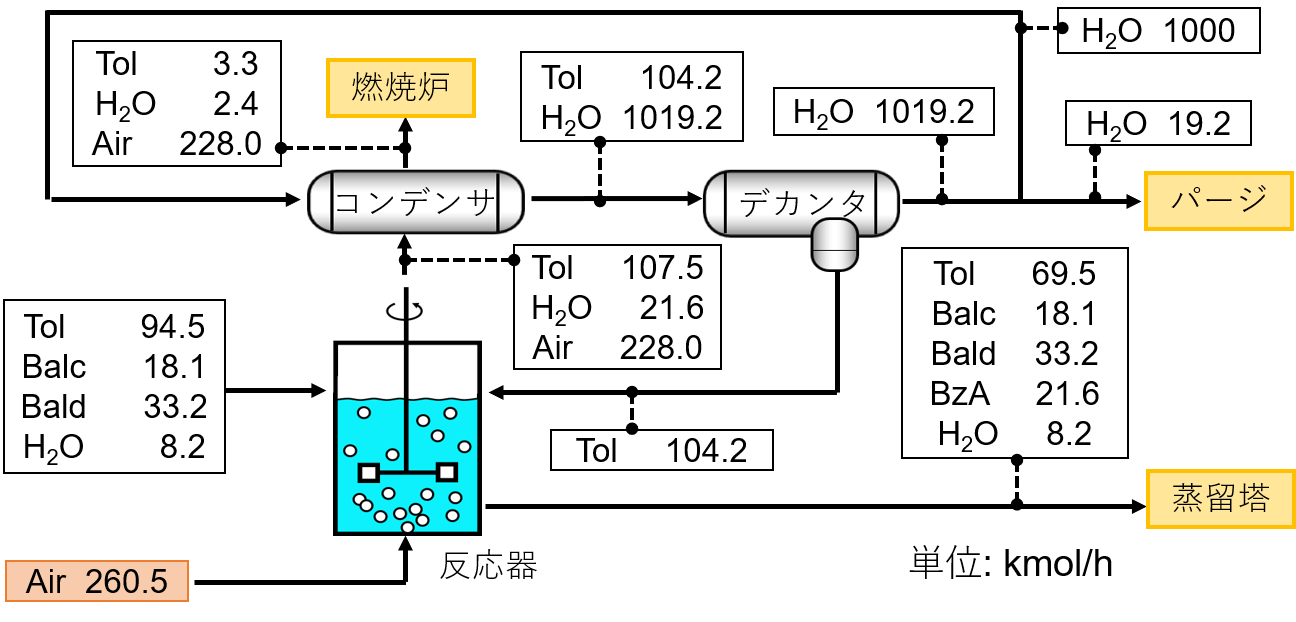
\includegraphics[scale=0.7]{ReactionSectionConclusion.png}
        \caption{反応部設計結果}
    \end{center}
\end{figure}

=======
    Eo = \frac{g \Delta \rho d_\mathrm{vs}^2}{\sigma}
\end{equation}

\section{反応器設計結果}
反応部の概略図および物質収支を以下に示す.
>>>>>>> miyamoto

\newpage
\chapter{分離部1}
\section{蒸留塔設計}
未反応トルエンのうち99\%以上を回収することを目的とした.
<<<<<<< HEAD
設計条件として,蒸留塔段数を10段,蒸留塔供給段は6段,還流比を1.0とした.

蒸留塔圧力を変更し,全体の利益を最大とする点について探索を行った.
反応器流出液圧力が7barであるため,最適な圧力であることが予想される.
蒸留塔の圧力を変化させ,人件費を除く全体の利益を評価関数としてプロットした
図\ref{蒸留塔圧力最適化}から,確かに7barで全体の利益が最大化されることを確認した.
\begin{figure}[htbp]
    \label{蒸留塔圧力最適化}
    \begin{center}
        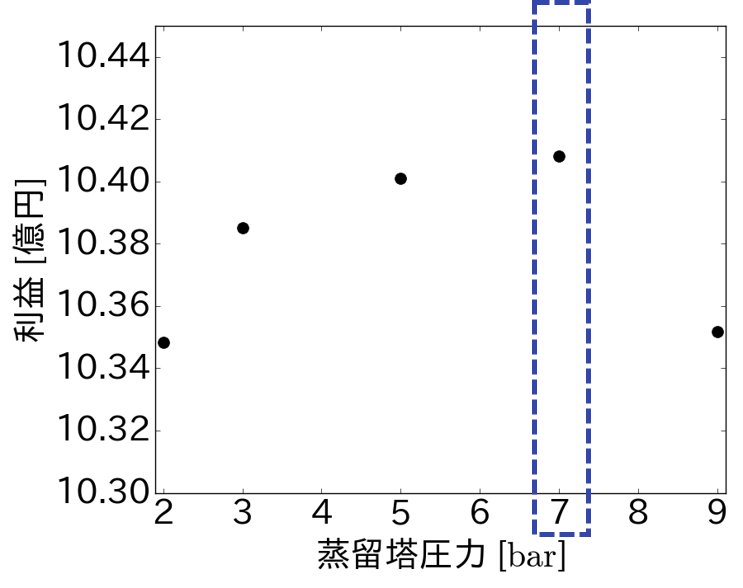
\includegraphics[scale=0.7]{DistillationPressue.png}
        \caption{蒸留塔圧力最適化}
    \end{center}
\end{figure}

設計結果を表\ref{蒸留塔設計結果}に記す.
\begin{table}[htbp]
    \label{蒸留塔設計結果}
    \caption{蒸留塔設計結果}
    \begin{center}
        \begin{tabular}{lc}
            \hline
            \multicolumn{1}{c}{項目} & 値 \\
            \hline
            塔径 \, [\si{\metre}] & 1.0 \\
            塔高 \, [\si{\metre}] & 6.1 \\
            塔内圧力 \, [\si{\bar}] &7 \\
            コンデンサ内温度 \, [\si{\degreeCelsius}] & 232 \\
            リボイラー内温度 \, [\si{\degreeCelsius}] & 316 \\
            \hline
        \end{tabular}
    \end{center}
\end{table}

\section{分離部1設計結果}
最適化後の最終結果における分離部1の流量関係を図\ref{分離部1設計結果の図}中に示す.
\begin{figure}[htbp]
    \label{分離部1設計結果の図}
    \begin{center}
        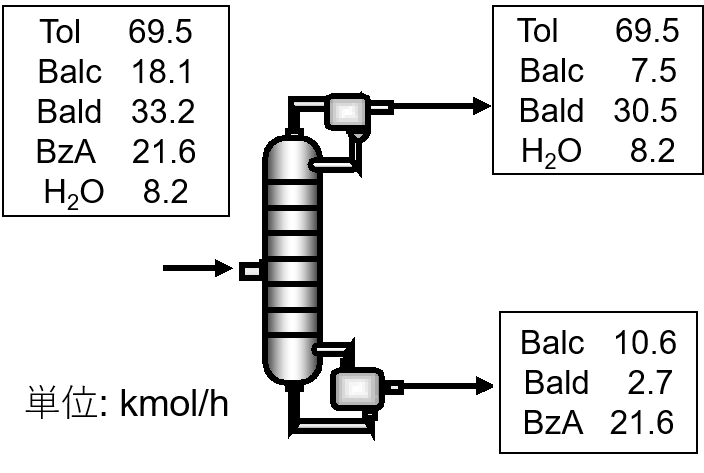
\includegraphics[scale=0.7]{Separation1Conclusion.png}
        \caption{分離部1設計結果}
    \end{center}
\end{figure}


\newpage
\chapter{分離部2}

=======
設計条件を以下に記す.

設計結果を以下に記す.

蒸留塔圧力を変更し,全体の利益を最大とする点について探索を行った.
反応器流出液圧力が7barであるため,最適な圧力であることが予想されるが,下記の
グラフに示されるように,確かに7barで全体の利益が最大化されることを確認している.

\newpage
\chapter{分離部2}
\section{晶析器設計}
>>>>>>> miyamoto
\section{晶析器選定}
溶解度の温度依存性が大きいことと,目的とする結晶生産量が大きいことから,
連続式攪拌槽型反応装置を選定した.\\
溶解度の温度依存性の相関式
\begin{equation}
    C^*=2.03\times 10^{-5}T^4 +2.03^{-5}\times T^4 + 2.97\times 10^{-4}T^3 + 4.70\times 10^{-2}T^2
        + 1.43T + 24.71
\end{equation}
<<<<<<< HEAD
ただし,温度$T \, [\si{\degreeCelsius}]$, $C^* \, [\si{\gram \per \kilo \solventgram}]$\\
\begin{figure}[htbp]
    \label{溶解度の温度依存性}
    \begin{center}
        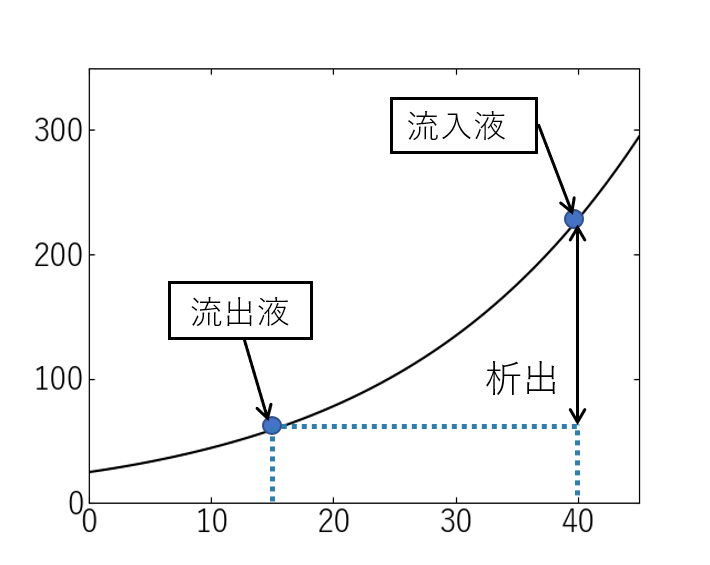
\includegraphics[scale=0.7]{BzAsolvent.png}
        \caption{溶解度の温度依存性}
    \end{center}
\end{figure}

=======
ただし,$T[\mathrm{^\circ C}]$,$C^*[{\mathrm g/kg-solvent}]$\\
>>>>>>> miyamoto

\section{設計方程式}
以下の仮定を用いた.
\begin{itemize}
    \setlength{\parskip}{0pt}
    \setlength{\itemsep}{2pt}
    \item[-] 結晶表面拡散は迅速に行われる.
    \item[-] 晶析器内は完全混合状態である.
    \item[-] 二次核発生の影響は無視する.
\end{itemize}

参考文献\cite{晶析}により,以下の実験式および理論式を用いて設計を行った.\\
一次核発生速度
\begin{equation}
    B^0 = k_\mathrm{b} M_\mathrm{T}^j \Delta C^b
\end{equation}
結晶成長速度
\begin{equation}
    G = k_\mathrm{g}\Delta C^g
\end{equation}
結晶成長速度定数
\begin{equation}
    k_\mathrm{g} = k_\mathrm{g0} \exp \left( -\frac{E_\mathrm{g}}{RT} \right)
\end{equation}
個数収支式
\begin{equation}
    n=n^0 \exp \left( -\frac{L}{G\tau} \right)
\end{equation}
懸濁密度
\begin{equation}
    M_\mathrm{T} = c_0-c = 6k_\mathrm{v} \rho_\mathrm{c} n^0 (G\tau)^4
\end{equation}
各パラメータは以下の通りである.
\begin{align*}
<<<<<<< HEAD
    &k_\mathrm{g0} = 1.06\times10^7 \, \si{(\micro \meter)/(\gram / \solventgram)^{\textit{g}}} \\
    &B^{\mathrm{0}} = 40.05 \, \si{\kilo \joule / \mole} \\
    &k_\mathrm{b} = 9.16 \times 10^{12} \, \si{(\# / \cubic \meter \second) / \{ (\gram / \milli \liter)^{\textit{j}} (\gram / \solventgram)^{\textit{b}} \} } \\
=======
    &k_\mathrm{g0} = 1.06\times10^7 \, \si{(\micro \meter)/(\gram / \gram-solvent)^{\textit{g}}} \\
    &B^{\mathrm{0}} = 40.05 \, \si{\kilo \joule / \mole} \\
    &k_\mathrm{b} = 9.16 \times 10^{12} \, \si{(\# / \cubic \meter \second) / \{ (\gram / \milli \liter)^{\textit{j}} (\gram / \gram-solvent)^{\textit{b}} \} } \\
>>>>>>> miyamoto
    &g = 0.44 \\
    &j = 1.78 \\
    &b = 1.2 \\
    &k_\mathrm{v} = 0.1 \\
    &\rho_\mathrm{c} = 1.32 \, \si{\gram / \centi \metre \cubed}
\end{align*}

<<<<<<< HEAD
=======

>>>>>>> miyamoto
\section{晶析器設計結果}
最適化の結果によって得られた晶析器の設計結果を以下に記す.

\section{抽出塔設計}
十分に塔内へ液を滞留させることによって安息香酸を水中に飽和させることを目的とした.
<<<<<<< HEAD
十分なデータを得られなかったため,2時間の装置内滞留によって安息香酸がトルエン溶媒中に飽和し,
その他ベンジルアルコール,ベンズアルデヒドの溶解度については無視できると仮定した.

\section{分離部2設計結果}
\begin{figure}[htbp]
    \label{分離部2設計結果}
    \begin{center}
        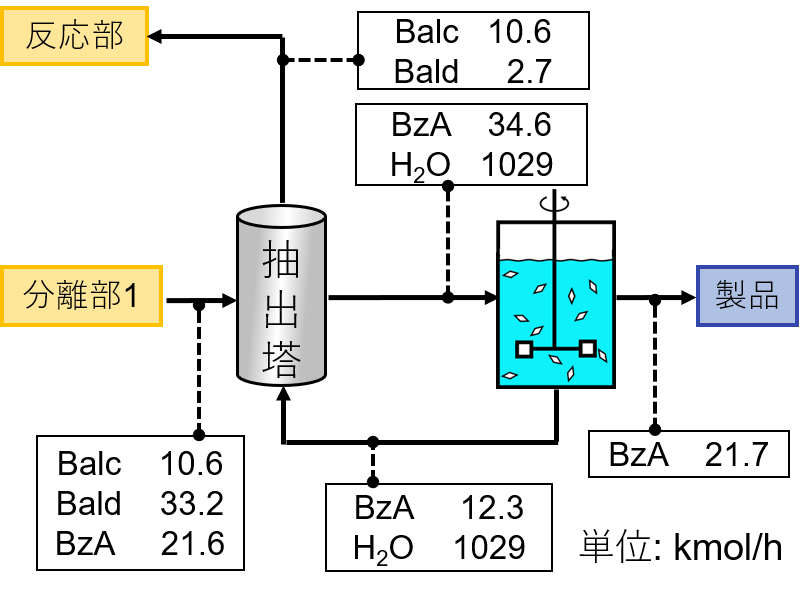
\includegraphics[scale=0.7]{Separion2Conclusion.png}
        \caption{分離部2設計結果}
    \end{center}
\end{figure}
=======
設計仮定を以下に記す.
設計条件を以下に記す.

>>>>>>> miyamoto

\newpage
\chapter{最適化}
\section{方法}
最適化を行うにあたり,最適化変数として以下の3つを選択した.
\begin{itemize}
  \item 反応器体積
  \item 晶析器体積
  \item 晶析器温度
\end{itemize}

これらの変数を選択した理由を述べる.反応器体積が大きいとき,反応器の装置コストは大きくなる.一方で,反応器出口から排出される未反応トルエンの量が減るため,蒸留塔のリボイラーで必要な熱量が減少し,熱煤のコストは減少する.反応器体積が小さいときは,反応器の装置コストは小さくなるが,熱煤のコストは大きくなる.晶析器体積が大きいとき,晶析器の装置コストは大きくなる.しかし,晶析する安息香酸の量が増えるため,リサイクルに回る安息香酸の量が少なくなり,それを保持するための純水の量が減少し,純水の費用は抑えられる.晶析器の体積が小さいときは,逆になる.晶析器温度が低い時,必要な外部冷媒の温度が低くなるため,冷媒の単価は高くなる.しかし,晶析する安息香酸の量が大きくなるため,リサイクルに回る安息香酸の量が小さくなり,必要な純水の量が減るため,純水を冷やすために用いている冷媒の量は小さく抑えられる.晶析器温度が高いときは,冷媒の単価は安くなるが,冷媒の必要量が大きくなる.このように,最適化変数に選択した変数は,その大小によって,なんらかのトレードオフの関係を生じる.そのため,これらの変数の値を変化させることで,利益が最大となる最適点を探索することが可能であると考えた.

次に,最適化の具体的な手法について述べる.プロセスを最適化するにあたり,3つの最適化変数変数全てを同時に最適化することを考えた.そこで,反応器体積は,$13.5 \sim 16.0 \, \si{\cubic \metre}$の範囲で6点,晶析器体積は,$6 \sim 12 \, \si{\cubic \metre}$の範囲で13点,晶析器温度は,$5.0 \sim 20.0 \, \si{\degreeCelsius}$の範囲で16点,計1248点のデータを取った.そして,それぞれのデータについてフィッティングを行った後に,それぞれの範囲を100当分し,データの個数を$100 \times 100 \times 100$点に増やした.それらのデータを用いて,横軸に晶析器温度,縦軸に晶析器体積を設定し,反応器体積の値を逐次的に変化させることで,100枚のヒートマップを作成した.ヒートマップが表す値は,
\begin{equation}
  \text{P.I.} = \text{(売上)} - \text{(原料コスト)} - \text{(装置コスト)} -\text{(用役コスト)}
\end{equation}
で表される評価関数の値とした.また,各ヒートマップ上で,評価関数の値が最大となる点をプロットした.さらに,そのプロットがどのように変化するかを見るために,横軸に反応器体積,縦軸に評価関数の値を取り,折れ線グラフを作成した.

\section{最適化結果}
<<<<<<< HEAD
評価関数の値が最大となった点での,ヒートマップおよび,評価関数の最大値の変化を表したグラフは図\ref{最適化結果}のようになった.また,作成したgifはgithubにアップしているので,興味のある方はご覧ください.\url{https://github.com/miyamo-sou/processdesign}
\begin{figure}[htbp]
    \label{最適化結果}
    \begin{center}
        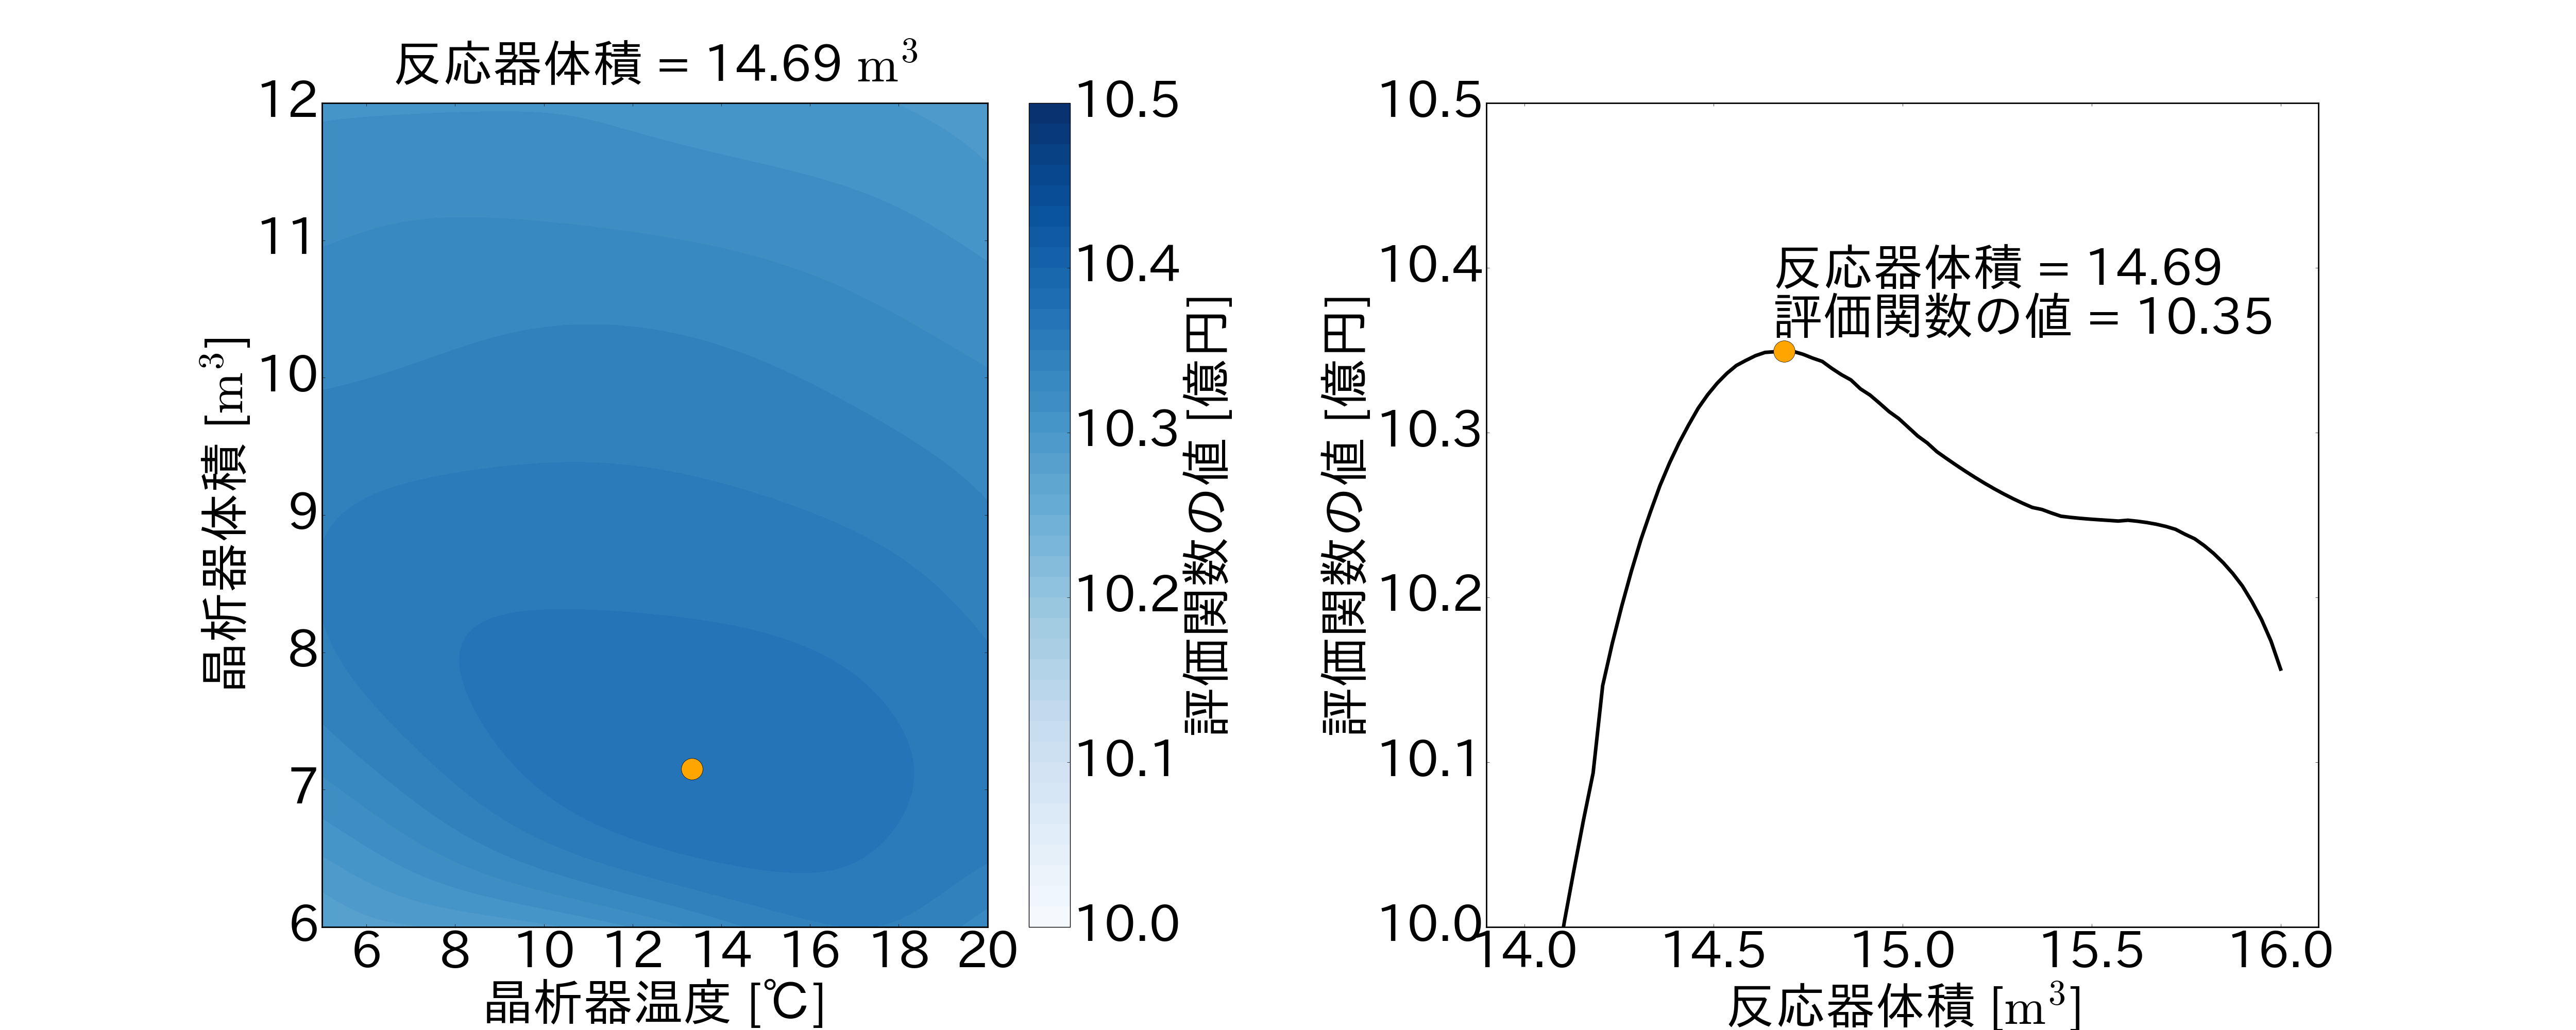
\includegraphics[scale=0.1]{snapshot.png}
        \caption{評価関数の値が最大となる点でのヒートマップと最適点の推移}
    \end{center}
\end{figure}

このよに,評価関数は大きなピークが存在する形になっていることが分かる.これは,最適化方法のセクションでも述べたが,反応器体積,晶析器体積,晶析器温度を変化させると,装置費と用役費がトレードオフの関係となって,コストが変化する.そのため,このようにピークが生じたと考えられる.
=======
評価関数の値が最大となった点での,ヒートマップおよび,評価関数の最大値の変化を表したグラフは図\ref{}のようになった.
>>>>>>> miyamoto


\newpage
\chapter{物質収支 $\cdot$ 熱収支}
全体のフロー図および流量関係は下図のようになった.

全体の熱量関係は以下のようになった.

\newpage
\chapter{ヒートインテグレーション}
流体同士の熱交換を行い,外部流体の利用量を削減した.
<<<<<<< HEAD
図\ref{TQ線図}に最終的な設計結果におけるTQ線図を示す.
\begin{figure}[htbp]
    \label{TQ線図}
    \begin{center}
        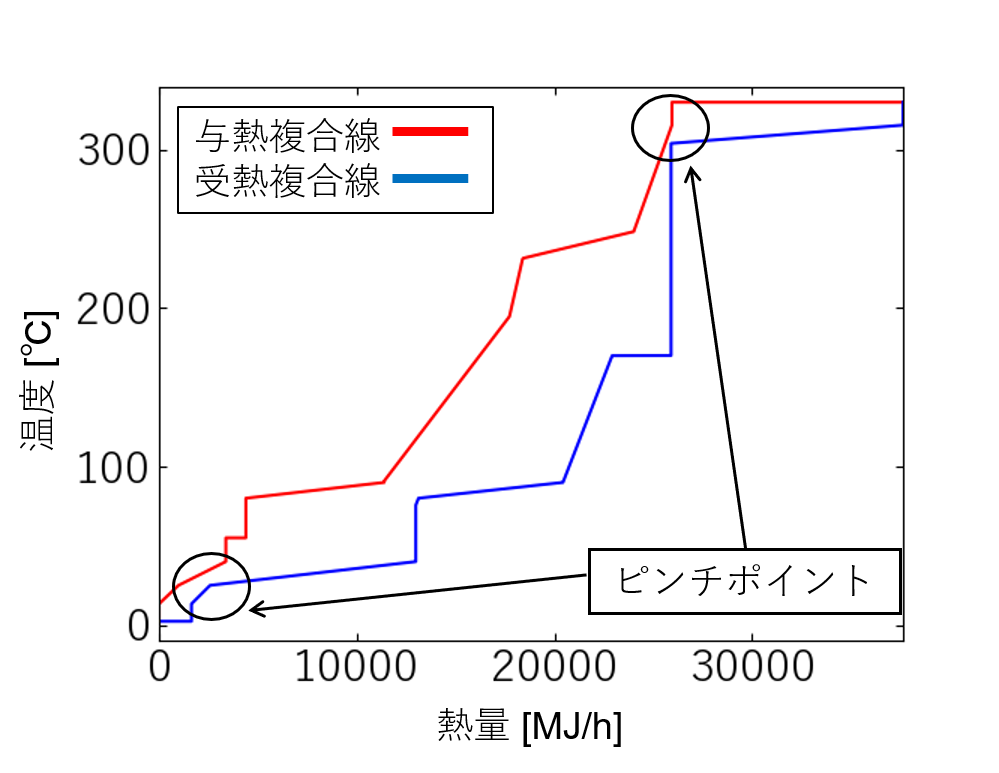
\includegraphics[scale=0.7]{TQdiagram.png}
        \caption{TQ線図}
    \end{center}
\end{figure}
=======
以下に最終的な設計結果におけるTQ線図を示す.
>>>>>>> miyamoto

熱交換により,外部熱媒を用いた場合と比較して,

\newpage
\chapter{経済評価}

\newpage
\chapter{結言}
設計目標を純度99.0wt\%の安息香酸を年2万ton製造するものとして,設計を行った.
<<<<<<< HEAD
文献値を参考として気液反応器,および晶析装置を設計した.
リサイクルフローを考えて,物質の有効利用を行った.
反応器体積,晶析器体積,晶析器内温度を用いたプロセス全体の3変数同時最適化を行った.
これにより,年 億円の利益を得ると見込める設計となった.
\par
残った課題としては,蒸発トルエンのさらなる回収を行うため,燃焼炉ではなく吸着装置を用いることを検討することや,
各装置についてさらに詳細に設計することが挙げられる.
=======
文献値を参考として反応器,および晶析装置を設計した.
また,リサイクルフローおよび燃焼炉の設置によって原料を有効活用できた.
最適化については,晶析器内温度および蒸留塔内圧力を順次最適化し,
プロセス全体について,反応器体積と晶析器体積を用いて最適化することができた.
本設計では積極的に多変数を用いて最適化を行った.
これにより,年 億円の利益を得ると見込める設計となった.
\par
課題としては,さらに多くの変数を用いた最適化,特に反応器内の条件を変更して行うこと,
また,燃焼炉ではなく,吸着装置を用いた時の比較検討を行うこと等が挙げられる.
>>>>>>> miyamoto

\newpage
\chapter*{謝辞}
\addcontentsline{toc}{chapter}{謝辞}
今回のプロセス設計では,様々な方々にお世話になりました.山本教授,谷口准教授を
はじめとする多くの化学工学の先生方,集中講義を実施してくださった玉川先生に感謝の意を申し上げます.
\par
また,1講座の先輩方の協力無しには私たちのプロセス設計は実現できませんでした.
プロセスの内容や発表に対し,的確なアドバイスをいただきました.
お忙しい中,原稿やスライドのチェック,発表練習などに協力して頂いたことで,無事に発表を終えることができました.
\par
私たちのプロセス設計に協力してくださった先生方,先輩方に改めて御礼申し上げます.

\newpage
<<<<<<< HEAD
\newpage
\bibliography{bibs/refs.bib}
\begin{thebibliography}{10}
    \bibitem{化工便覧} 化学工学便覧・化学工学会・丸善出版
    \bibitem{晶析} Gary Morris and  Graham Power \textit{et al.  Org. Process Res. Dev.} \textbf{19}, 1891-1902, 2015
    \bibitem{キー} 参考文献の名前・著者N
\end{thebibliography}
=======
\bibliography{bibs/refs.bib}
>>>>>>> miyamoto

\newpage
\chapter*{変数一覧}
\addcontentsline{toc}{chapter}{変数一覧}
\begin{multicols}{2}
\begin{flushleft}
  $a : \text{比界面積}$ \\
  $B^0 : \text{一次核発生速度}$ \\
  $c : \text{重量濃度}$ \\
  $C : \text{モル濃度}$ \\
  $C_\mathrm{D} : \text{抗力係数}$ \\
  $D : \text{拡散係数}$ \\
  $d_\mathrm{vs} : \text{気泡体積平均径}$ \\
  $E : \text{活性化エネルギー}$ \\
  $E_\mathrm{g} : \text{結晶化過程の活性化エネルギー}$ \\
  $F : \text{モル流量}$ \\
  $g : \text{重力加速度}$ \\
  $G : \text{核成長速度}$ \\
  $k : \text{反応速度定数}$ \\
  $k_\mathrm{b} : \text{核発生速度定数}$ \\
  $k_\mathrm{g} : \text{核成長速度定数}$ \\
  $k_\mathrm{L} : \text{液相物質移動係数}$ \\
  $k_\mathrm{L} a : \text{液相物質移動容量係数}$ \\
  $k_\mathrm{v} : \text{結晶体積形状係数}$ \\
  $M_\mathrm{T} : \text{懸濁密度}$ \\
  $n : \text{結晶の個数密度}$ \\
  $P_\mathrm{G} : \text{攪拌動力}$ \\
  $P_\mathrm{T} : \text{}$ \\
  $r : \text{反応速度定数}$ \\
  $T : \text{温度}$ \\
  $T_\mathrm{c} : \text{臨界温度}$ \\
  $u_\mathrm{t} : \text{気泡の終末速度}$ \\
  $u_\mathrm{G} : \text{気泡の空塔速度}$ \\
  $V : \text{体積}$ \\
  $\beta : \text{還流率}$ \\
  $\mu : \text{粘度}$ \\
  $\mu_\mathrm{L} : \text{液相粘度}$ \\
  $\sigma : \text{界面張力}$ \\
  $\rho_\mathrm{a} : \text{空気密度}$ \\
  $\rho_\mathrm{L} : \text{液相密度}$ \\
  $\rho_\mathrm{g} : \text{気相密度}$ \\
  $\varDelta\rho : \text{密度差}$ \\
  $Eo : \text{エトベス数}$ \\
  $Sc : \text{シュミット数}$ \\
  $Re : \text{レイノルズ数}$
\end{flushleft}
\end{multicols}

<<<<<<< HEAD

\chapter*{Appendix}
\addcontentsline{toc}{chapter}{Appendix}
=======
\newpage
\section*{Appendix}
>>>>>>> miyamoto

\end{document}
